\documentclass[10pt,a4paper]{article}
\usepackage[utf8]{inputenc}
\usepackage[T1]{fontenc}
\usepackage{graphicx}
\title{
Programming Assignment 3:
Implementing TAS, CAS and Bounded Waiting CAS
Mutual Exclusion Algorithms }
\author{CS21BTECH11055 - SADINENI ABHINAY}
\begin{document}
	\maketitle
	\section{Aim and Intro:}
	\subsection{Aim:}
	To implement and compare the perforamcse of TAS,CAS,Bounded CAS Mutual Exculsion Algorithims
	\subsection{Intro}
	\begin{enumerate}
		\item \textbf{Test and set:}\\
		 The test and set() instruction sets the lock true and returns the pre updated value of the lock 
		 The important characteristic of this instruction is that it is executed atomically. if the pre-updated value of lock is 0 that means the thread can enter the critical section.
		 Thus, if two test and set() instructions are executed simultaneously
		 (each on a different core), they will be executed sequentially in some arbitrary
		 order.
		 \item \textbf{Compare and swap:}\\
		 The compare and swap() instruction (CAS), just like the test and set()
		 instruction, operates on two words atomically, but uses a different mechanism that is based on swapping the content of two words.Regardless, CAS always returns the original value of
		 the variable value. The important characteristic of this instruction is that it is
		 executed atomically. Thus, if two CAS instructions are executed simultaneously
		 (each on a different core), they will be executed sequentially in some arbitrary
		 order.
		 \item \textbf{Bounded Waiting Compare and swap:}\\
		 A process can enter critical section only when it is not waiting and the lock is open.The first process to execute the compare and swap will find key value 0,which is 1 when found by other processes so they will wait.the waiting of only one processes is set to false when it exits the critical section which maintains mutual exclusion requirement.To prove that the bounded-waiting requirement is met, we note that, when process leaves the 
		 critical section it scans the waiting array and designates the the first process in cyclic ordering.Any process which is waiting will enter the critical section within n-1 turns. 
		
	\end{enumerate}

\section{Performance analysis:}
 \subsection{Average Time Taken:}
 \begin{figure}[!ht]
 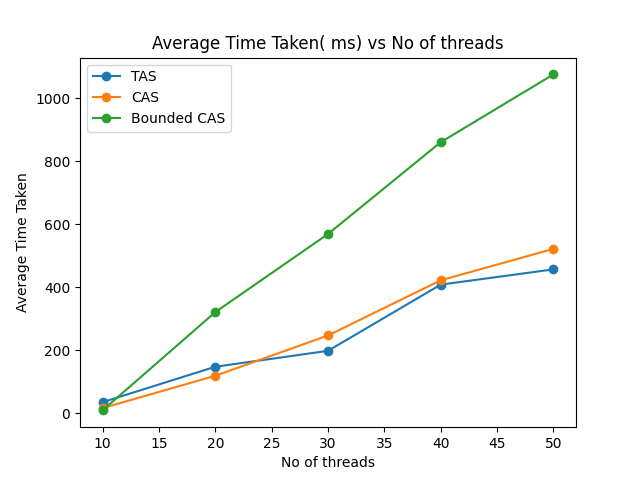
\includegraphics[scale = 0.8]{fig1}
 \label{}
 \caption{Average Time Taken v/s No of threads}
\end{figure}
\textbf{Observations:}
\begin{enumerate}
	\item As seen above the average is highest for bounded Waiting CAS algorithm  compared to TAS and normal CAS. This is because the thread scans the waiting array for
	which are ready or starving for Critical section. The extra search overhead is more.  
	\item CAS and TAS are surprisingly has similar average this is because the operation may be different but both are changing lock
	\item Overall the trend is as excepted ,the average increases with increase in number of threads because later thread needs to wait for more time to enter the critical section.
	\item We can conclude that TAS and CAS are better when compared average,but 
	Let see another merit of Bounded CAS in next plot.
\end{enumerate}
\pagebreak
\subsection{Worst Time Taken:}
 \begin{figure}[!ht]
	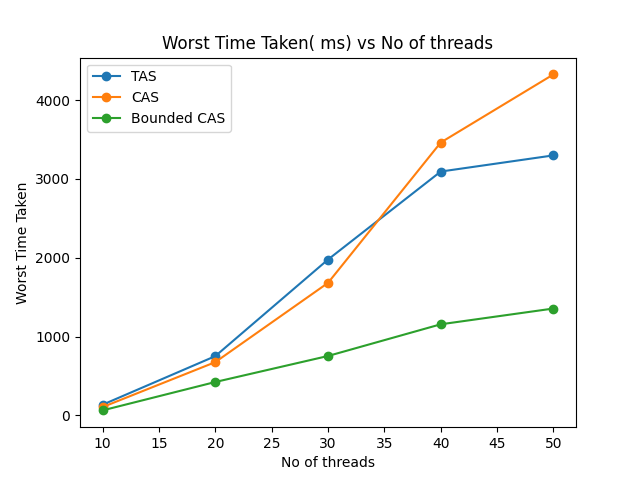
\includegraphics[scale = 0.8]{fig2}
	\label{}
	\caption{Worst Time Taken v/s No of threads}
\end{figure}
\textbf{Observations:}
\begin{enumerate}
	\item Bounded Waitng CAS has least Worst time among all the three algorithm this is beacuse the it takes care of the starving threads  by running a cyclic search after a thread exits critical section which reduces the waiting time of thread in the entry section
	\item CAS and TAS are surprisingly has similar worst this is because the operation may be different but both are changing lock still At n=50 CAS has more worst time due some extra time spent on comparing lock value(less significant).  
	\item Overall the trend is as excepted ,the worst case increases with increase in number of threads because the last thread needs to wait for more time to enter the critical section.
	\item Bounded Waiting CAS ensures less starvation for threads comapred to TAS and CAS.
\end{enumerate}

\end{document}